\chapter{Estado del Arte}
\label{ch:sota}

Este capítulo tiene como objetivo principal revisar los conceptos clave y el estado del arte que constituyen la base de esta tesis. Para ello, se ha estructurado el capítulo en tres grandes bloques. En primer lugar, se explorarán las redes programables y softwarizadas partiendo de las redes \gls{sdn}, se seguirá con los algoritmos de red y el uso de la \gls{ai} como tecnologías habilitadoras, y por último, se analizarán diversos casos de uso relevantes que ejemplifican la aplicación práctica de estas tecnologías, como son las \gls{sg} y las redes de sensores \gls{iiot}. 

\section{Las redes \glsentryshort{sdn}}
\label{sec:redes_sdn} 

En este primer bloque se revisan las redes \gls{sdn}, que son la base de las redes programables y softwarizadas. Se explorarán sus características, ventajas y desventajas, así como sus paradigmas de modos de control, según se indicó anteriormente. Además, se analizarán los protocolos y así como los aspectos clave de las vertientes de trabajo del modo de control \textit{in-band}, y cómo podemos explorar dicho modo para favorecer la flexibilidad y control en redes densas y heterogéneas.\\
\\
Las redes definidas por software (\gls{sdn}) representan un nuevo paradigma que rompe con las arquitecturas tradicionales de red. Antes de que apareciera el concepto de \gls{sdn}, como se puede apreciar en la Figura~\ref{fig:sdn_paradigma}, las redes tradicionales solían tener un plano de control unificado en los propios dispositivos, llamado generalmente \textit{Control plane}, en el que se definía la lógica que dictaba cómo se debía llevar a cabo el forwarding de los paquetes, y un plano de datos, conocido como \textit{Data plane}, que se implementaba definiendo su datapath, compuesto por varios bloques de procesamiento para reenviar los paquetes. Ambos planos estarían unificados en un sentido lógico, en un mismo dispositivo. Sin embargo, con la aparición del paradigma de las redes \gls{sdn}, como se muestra en la Figura, los nodos tradicionales de la red verían cómo su plano de control sería delegado a una entidad externa llamada controlador, preserbando su capadicar para manejar los paquetes. En contratste con las arquitecturas tradicionales de la red, donde había que ir configurando equipo a equipo, y donde cada uno de ellos iba a desempeñar una función de red, en las redes \gls{sdn}, el controlador permite configurar y supervisar de manera inteligente el comportamiento de la red a través de aplicaciones software, facilitando una programación flexible y dinámica del entorno de red. Por lo que, aunque se sigan llamando ``switches'' o nodos \gls{sdn}, estos se comportarán según las reglas que le instale el controlador, pudiendo gestionar paquetes como un switch, un router, un firewall, etc. 

\begin{figure}[ht!]
\centering
\includegraphics[width=\textwidth]{fig/02_sota/sota_1_sdn_idea.drawio.pdf}
\caption{Paradigma en las redes \glsentryshort{sdn}}
\label{fig:sdn_paradigma}
\end{figure}

La centralización de la gestión simplifica notablemente las tareas del administrador, al proporcionar una visión global del estado de la red y un punto único desde el cual definir su funcionamiento. A través del controlador, las complejas instrucciones de bajo nivel requeridas por los dispositivos de red tradicionales, como switches y routers, las cuales podían variar en función del fabricante, se abstraen mediante interfaces con sintaxis intuitiva, reduciendo la complejidad operativa. Estas capacidades dotan a la red de una gran agilidad y capacidad de adaptación ante cambios o nuevas necesidades, pudiendo conmutar entre distintos perfiles de funcionamiento de forma automática. El simple despliegue de una nueva aplicación sobre el controlador permite modificar de forma coherente el comportamiento de toda la infraestructura, disminuyendo así los costes asociados al mantenimiento, la operación y el despliegue. Además, SDN promueve activamente el uso de soluciones abiertas tanto a nivel de software como de hardware, fomentando ecosistemas interoperables, reduciendo la dependencia de tecnologías propietarias y eliminando barreras de entrada para nuevos actores en el sector.

\subsection{Arquitectura lógica de las redes \glsentryshort{sdn}}
\label{subsec:arquitectura_sdn}

La arquitectura lógica de las redes \gls{sdn} se puede dividir en dos planos, el plano de control y el plano de datos, y además, en tres capas: capa de aplicación, capa de control y capa de infraestructura. En la Figura~\ref{fig:sdn_architecture} se muestra la arquitectura lógica de las redes \gls{sdn}, así como sus interfaces principales de comunicación que más adelante se explicarán.\\
\\
El plano de control, se estructura internamente en dos capas funcionales: la capa de control y la capa de aplicación. Estas se comunican mediante la interfaz norte (northbound interface), que permite a las aplicaciones definir políticas de alto nivel que serán interpretadas y gestionadas por el controlador. Estas capas a menudo se pueden encontrar corriendo en la misma máquina, donde conviven el controlador y las aplicaciones que interactúan con él. Sin embargo, también se puede tener un enfoque distribuido, donde el controlador está en una, máquina, y las aplicaciones en otra, haciendo uso de la interfaz northbound. Por su parte, el plano de datos está conformado por la capa de infraestructura, que engloba los dispositivos físicos de red, principalmente switches \gls{sdn}, responsables del reenvío de paquetes. La interacción entre el plano de control y el plano de datos se realiza a través de la interfaz sur (southbound interface), cuya función es traducir las decisiones del plano de control en instrucciones ejecutables por los dispositivos de red. En este contexto, el controlador actúa como una pieza clave del sistema, asumiendo responsabilidades esenciales como la instalación de reglas de encaminamiento, la monitorización continua del estado de la red y la recopilación de métricas operativas, las cuales serán aprovechadas por todas las aplicaciones que se ejecuten sobre el controlador.

\begin{figure}[ht!]
\centering
\includegraphics[width=0.5\textwidth]{fig/02_sota/sota_2_sdn_arch_b.drawio.pdf}
\caption{Arquitectura lógica de las redes \glsentryshort{sdn}}
\label{fig:sdn_architecture}
\end{figure}

El plano de datos, por el contrario, no posee lógica de control propia, limitándose a ejecutar las reglas recibidas, como por ejemplo, hacer un reenvío, o descartar paquetes según las reglas establecidas, además de  enviar estadísticas de tráfico al controlador. Esta separación de funciones establece una división clara entre la inteligencia de la red, localizada en el plano de control, y su ejecución, delegada como se ha explicado, al plano de datos. De esta manera, se rompe con el modelo tradicional en el que ambos planos coexistían en un mismo dispositivo de red. Este enfoque modular no solo mejora la escalabilidad y la flexibilidad del sistema, sino que también reduce significativamente los costes de despliegue (\gls{capex}) y operación (\gls{opex}), al concentrar los recursos de cómputo en un nodo centralizado, y simplificar el hardware requerido en los dispositivos de reenvío.\\
\\
Según se ha visto en la Figura~\ref{fig:sdn_architecture}, la arquitectura \gls{sdn} se apoya en una estructura jerárquica formada por tres capas principales: aplicación, control e infraestructura. La capa de aplicación representa el nivel de mayor abstracción dentro del ecosistema \gls{sdn}. Esta capa integra un conjunto de aplicaciones que, apoyándose en los servicios ofrecidos por la capa de control, permiten definir políticas de gestión, \gls{qos}, optimizar el rendimiento de la red y adaptarla dinámicamente a diferentes contextos operativos. Un ejemplo típico de uso es la utilización los servicios de descubrimiento topológico proporcionados por la capa de control, que permiten a las aplicaciones calcular rutas óptimas entre dispositivos de red. Estas aplicaciones suelen desarrollarse empleando lenguajes de alto nivel como Python, Go o C++, con el objetivo de facilitar su portabilidad entre plataformas y maximizar la reutilización del código. No obstante, en la práctica, la existencia de \glspl{api} y entornos de desarrollo específicos para cada plataforma de control, como ONOS, OpenDaylight, Ryu o el nuevo controlador del ecosistema \gls{sdn}, TeraflowSDN, introduce ciertos desafíos en la interoperabilidad y portabilidad del software entre distintas implementaciones. En este sentido, uno de los principales retos actuales de \gls{sdn} sigue siendo la estandarización de interfaces northbound que permitan una integración más fluida y flexible entre aplicaciones y controladores heterogéneos.\\
\\
Descendiendo, la siguiente capa es la capa de control, la cual constituye el núcleo funcional del paradigma \gls{sdn}, albergando la inteligencia centralizada de la red. Actúa como intermediario entre las aplicaciones de alto nivel y los dispositivos físicos de la capa de infraestructura, orquestando tareas críticas como el encaminamiento de flujos, la detección y resolución de fallos, la supervisión continua del estado de la red y la gestión de políticas de seguridad y \gls{qos}. Su papel como middleware se traduce en la capacidad de transformar políticas abstractas generadas en la capa de aplicación en instrucciones simples y concretas que pueden ser entendidas por los nodos \gls{sdn}. Esta capacidad de traducir y escalar la lógica de red permite que un único controlador gobierne cientos o miles de switches de forma eficiente, garantizando escalabilidad y consistencia en entornos distribuidos. Por último, la capa de infraestructura, por su parte, está compuesta por los elementos físicos de la red, fundamentalmente nodos \gls{sdn}, que ejecutan las decisiones tomadas por el plano de control. Estos dispositivos, carentes de lógica propia, cuentan con un agente \gls{sdn} encargado de comunicarse con el controlador a través de la interfaz sur (southbound interface), como por ejemplo, OpenFlow o P4Runtime. Su funcionalidad se reduce al reenvío y descarte de paquetes o la recolección de estadísticas, lo que permite simplificar su diseño y reducir sus requisitos hardware.\\
\\
En cuanto a las interfaces, hay dos, como se ha mencionado anteriormente, la interfaz northbound y la interfaz southbound. La interfaz northbound constituye el canal de comunicación entre la capa de control y la capa de aplicación. Su principal función es ofrecer un punto de acceso lógico al administrador de red, permitiéndole supervisar, configurar y gestionar el comportamiento de la red sin necesidad de interactuar directamente con los mecanismos de bajo nivel que gobiernan los dispositivos físicos. A través de esta interfaz, las aplicaciones pueden programar políticas o solicitudes que serán traducidas por el controlador en instrucciones comprensibles para los elementos de la infraestructura. No obstante, a diferencia de la interfaz southbound, la interfaz northbound carece de una estandarización formal. En consecuencia, la naturaleza y funcionalidad de esta interfaz varían considerablemente en función del controlador \gls{sdn} empleado, cada uno de los cuales suele ofrecer su propia \gls{api} con diferentes modelos de datos, protocolos y lenguajes de interacción.\\
\\
La interfaz southbound constituye el enlace entre la capa de control y la capa de infraestructura dentro de una arquitectura \gls{sdn}. A diferencia de la interfaz northbound, esta sí cuenta con protocolos estandarizados ampliamente adoptados, que permiten la interoperabilidad entre los controladores y los dispositivos de red. Históricamente, el protocolo más representativo ha sido Openflow~\cite{mckeown2008openflow}. En la implementación del protocolo Openflow según se indica en la Figura~\ref{fig:sdn_openflow}, el concepto central es el de flujo (del inglés, \textit{flow}), entendido como un conjunto de paquetes que cumplen determinadas condiciones definidas por el controlador. Estas condiciones se almacenan en las denominadas tablas de flujo (del inglés, \textit{flow tables}), y suelen hacer referencia a valores específicos de campos en la cabecera del paquete o al puerto de entrada por el que se ha recibido.

\begin{figure}[ht!]
\centering
\includegraphics[width=0.7\textwidth]{fig/02_sota/sota_3_sdn_openflow.drawio.pdf}
\caption{Arquitectura básica de switch OpenFlow}
\label{fig:sdn_openflow}
\end{figure}

Cuando un paquete llega a un switch Openflow, empieza a atravesar de forma iterativa las tablas de flujo y cuando este coincide con los criterios de una regla definida en una tabla, se produce una coincidencia (del inglés, \textit{match}), lo que activa un conjunto de instrucciones asociadas a dicha regla. Estas instrucciones pueden incluir el conteo de paquetes, la aplicación de acciones concretas (como reenviar o descartar el paquete), o bien su reenvío hacia otra tabla para un procesamiento adicional. En caso de no darse una coincidencia, se encapsula y se manda al controlador para que este decida que cómo manejarlo. Así, mediante la instalación de estas reglas por parte del controlador \gls{sdn}, se determina el comportamiento de reenvío del switch. La comunicación entre el controlador y los dispositivos se realiza a través de un canal estructurado y seguro, que admite mensajes del controlador al switch, mensajes asíncronos generados por los dispositivos, y mensajes simétricos intercambiables por ambas partes, permitiendo una gestión eficiente y dinámica del estado de red.\\
\\
No obstante, las limitaciones de flexibilidad, extensibilidad y adaptación a nuevas arquitecturas han motivado el surgimiento de alternativas a Openflow. Un ejemplo destacado es el lenguaje \gls{p4}~\cite{bosshart2014p4}, diseñado específicamente para superar las restricciones de OpenFlow. Una de las mayores restricciones que tiene OpenFlow es la especificación de forma explícita de los campos de cabecera sobre los que opera. Estos campos de cabecera han pasado de 12 a 41 campos de cabeceras entre sus versiones 1.0 y 1.5 como se puede ver en la Tabla~\ref{tab:openflow_versions}. Esta evolución ha incrementado la complejidad del protocolo sin proporcionar la flexibilidad necesaria para incorporar nuevas cabeceras o funcionalidades emergentes. 

\begin{table}[ht!]
\centering
\begin{tabular}{|c|c|l|}
\hline
\textbf{Versión} & \textbf{Fecha} & \textbf{Campos de cabecera} \\ \hline
OF 1.0 & Dic. 2009 & 12 campos (Ethernet, TCP/IPv4) \\ \hline
OF 1.1 & Feb. 2011 & 15 campos (MPLS, metadatos entre tablas) \\ \hline
OF 1.2 & Dic. 2011 & 36 campos (ARP, ICMP, IPv6, etc.) \\ \hline
OF 1.3 & Jun. 2012 & 40 campos \\ \hline
OF 1.4 & Oct. 2013 & 41 campos \\ \hline
OF 1.5 & Mar. 2015 & 44 campos \\ \hline
\end{tabular}
\caption{Evolución de versiones del protocolo Openflow y el número de campos de cabecera soportados}    
\label{tab:openflow_versions}
\end{table}

En respuesta a ello, \gls{p4} nació con tres objetivos principales: 

\begin{itemize}
    \item Permitir la reconfiguración del dispositivo en caliente, es decir, cambiar el comportamiento de los switches una vez desplegados.
    
    \item Ofrecer independencia de protocolo, desvinculando el procesamiento de paquetes de protocolos específicos que tengan que estar estandarizados para poder ser gestionados.
    
    \item Proporcionar independencia del hardware, permitiendo que las funcionalidades de procesamiento se definan sin depender de los detalles del dispositivo subyacente. Si bien es cierto que la iniciativa de \gls{p4} nació con este objetivo en mente (\textit{open-hardware}), la realidad es que, en la actualidad, se ha visto como cada fabricante ha implementado equipos que si cumplen con algunas de las arquitecturas de \gls{p4}, pero que cada uno te ofrece unas primitivas de programación diferentes, haciendo que un programa \gls{p4} que corre en un dispositivo de un fabricante no sea totalmente compatible en otro~\cite{hauser2023survey}. 
\end{itemize}

En comparación con Openflow, si nos fijamos en la Figura~\ref{fig:sdn_p4}, podemos apreciar que empleando \gls{p4} se puede definir el cómo el switch va a manejar los paquetes, como los va a procesar y parsear, manteniendo la lógica de las tablas de flujo que teníamos en Openflow, pero ganando en flexibilidad dado que se pueden definir el propio datapath del dispositivo sin depender de un conjunto estandarizado de campos de cabecera. Esto incluso permite que \gls{p4} pueda ser implementado en dispositivos de baja capacidad~\cite{carrascal2020analysis}, al poder ajustar el datapath a la mínima expresión necesaria para cumplir con las necesidades de la red. Al igual que en Openflow se tenía el protocolo de comunicación para la interfaz southbound, \gls{p4} también tiene su propia interfaz de comunicación, llamada P4Runtime~\cite{p4runtime2023}, que permite a los controladores gestionar y programar dispositivos \gls{p4} de forma dinámica. 

\begin{figure}[ht!]
\centering
\includegraphics[width=0.9\textwidth]{fig/02_sota/sota_4_sdn_p4.drawio.pdf}
\caption{Arquitectura básica de switch \glsentryshort{p4}}
\label{fig:sdn_p4}
\end{figure}

A diferencia de Openflow, que define un conjunto cerrado de operaciones y estructuras, \gls{p4} y su interfaz P4Runtime introducen la posibilidad de reconfigurar dinámicamente el comportamiento del plano de datos mediante descripciones personalizadas del procesamiento de paquetes. Esto se logra mediante una arquitectura basada en \gls{grpc}, que ofrece cinco tipos de operaciones principales (Write, Read, Set/GetForwardingPipelineConfig y StreamChannel) para gestionar tanto el estado como la lógica interna de los switches programables. De esta forma, \gls{p4} se presenta como una propuesta de evolución de Openflow, orientada a lograr una programabilidad del plano de datos más flexible y escalable, haciéndolo ideal para testing y pruebas de concepto de nuevas soluciones de red.\\
\\
Paralelamente, ha ido creciendo otra vía complementaria orientada a la gestión y configuración unificada de dispositivos de red llamada OpenConfig. Esta iniciativa, impulsada mayormente por un consorcio de operadores y fabricantes, propone un conjunto de modelos de datos basados en YANG que permiten describir de forma estandarizada y agnóstica el estado operativo y la configuración de dispositivos de red. A diferencia de OpenFlow o P4Runtime, que se centran en el comportamiento del plano de reenvío, OpenConfig aborda la gestión, configuración, el monitoreo y la automatización de tareas de red a través de protocolos como gNMI o NETCONF. Esto convierte a OpenConfig una herramienta clave para aquellas empresas que buscan una gestión softwarizada y programable de sus infraestructuras ya existentes, dado que permite la integración de dispositivos heterogéneos de diferentes fabricantes bajo un modelo común de gestión. Si bien es cierto que OpenConfig no permite definir explícitamente el plano de datos, a diferencia de Openflow o \gls{p4}, donde se considera que todos los switches o nodos \gls{sdn} equivalen a un único dispositivo lógico gestionado de forma centralizada, OpenConfig propone un enfoque diferente. Esta iniciativa busca establecer un conjunto común de modelos de datos y configuración, independientes del fabricante, para gestionar redes heterogéneas. A diferencia del enfoque \gls{sdn} tradicional, en el que los dispositivos se integran como un único plano de control y datos, los dispositivos gestionados mediante OpenConfig siguen operando como entidades independientes. Ambos enfoques persiguen una mayor transparencia y facilidad de gestión de la red, pero difieren en su grado de abstracción y centralización: mientras \gls{sdn} trata la red como un todo unificado, OpenConfig mantiene la identidad individual de cada dispositivo, facilitando la interoperabilidad en entornos mixtos. Sin embargo, los últimos controladores \gls{sdn} como TeraflowSDN~\cite{teraflowsdn2021}, han comenzado a integrar OpenConfig como una de sus interfaces southboud (además de \gls{p4}), incluso llegando a no implementar Openflow, lo que sugiere una tendencia hacia un nuevo ecosistema de redes \gls{sdn} que combina la flexibilidad de la programación del plano de datos con la estandarización y la gestión eficiente de dispositivos heterogéneos.\\
\\
En este sentido, la evolución de la interfaz southbound no debe entenderse en términos de sustitución de unos protocolos por otros, sino como una diversificación funcional que permite combinar capacidades de reenvío programable, comunicación eficiente y gestión estandarizada según las necesidades específicas de cada red.


\subsection{Arquitectura física de las redes \glsentryshort{sdn}}
\label{subsec:arquitectura_fisica_sdn}

Una vez que se ha revisado la arquitectura lógica de las redes \gls{sdn}, es importante entender cómo se implementa físicamente esta arquitectura, es decir, cómo se conectan los diferentes componentes que se vienen explicando en la sección anterior.\\
\\
En una red \gls{sdn}, según se indicó en la Figura~\ref{fig:sdn_architecture}, se compone de un elemento central, el controlador, y un conjunto de swicthes o nodos \gls{sdn} distribuidos en la capa de infraestructura los cuales son gestionados por el controlador. Sin embargo, también es posible la implementación de múltiples controladores en una misma red \gls{sdn}, lo cual aporta funcionalidades adicionales a la red, como mecanismos de respaldo y tolerancia a fallos, que incrementan su fiabilidad, y por ende, la resilencia de la red. Por ello, se pueden clasificar las conexiones físicas en las redes \gls{sdn} en dos bloques:  

\begin{itemize}
    \item Las conexiones entre los switches de la capa de infraestructura.
    \item Las conexiones entre el controlador y los switches de la capa de infraestructura.
\end{itemize}
 
Las primeras constituyen la topología física de la red, cuya estructura depende del entorno en el que se despliegue y de los objetivos funcionales de la red. Por ejemplo, en redes \gls{sdn} diseñadas para centros de datos, es común adoptar una arquitectura jerárquica y regular, ya que esta facilita la escalabilidad y permite absorber incrementos en la demanda de tráfico de forma eficiente~\cite{lopez2021nuevos}. En cambio, en entornos de redes de sensores \gls{sdn}, es frecuente emplear topologías en malla parcial (tendiendo hacia a una malla completa)~\cite{baddeley2018evolving}, que permiten una mayor resiliencia frente a fallos y una reducción en la latencia gracias a la existencia de múltiples caminos entre nodos de la topología.\\
\\
En cuanto a las conexiones entre el controlador y los switches de la capa de infraestructura, estas se pueden clasificar en principalmente en dos categorías, si bien es cierto que se puede encontrar una tercera categoría que combina ambas. Observando la Figura~\ref{fig:sdn_control_paradigms}, se pueden distinguir dos paradigmas de control: el modo de control \textit{in-band} y el modo de control \textit{out-of-band}, y por último, el modo de control \textit{hybrid-band}, el cual es una combinación de los dos anteriores. \\

\begin{figure}[ht!]
\centering
\includegraphics[width=\textwidth]{fig/02_sota/sota_5_sdn_control_paradigms.drawio.pdf}
\caption{Paradigmas de control en las redes \glsentryshort{sdn}}
\label{fig:sdn_control_paradigms}
\end{figure}

Al desplegar el canal de control en una red \gls{sdn}, es posible optar por un enfoque out-of-band o in-band, como se ilustra en la Figura~\ref{fig:sdn_control_paradigms}. En el primer caso, denominado out-of-band, cada nodo \gls{sdn} dispone de un enlace físico dedicado que lo conecta directamente con el controlador. De este modo, la información de control se transmite a través de una red independiente, exclusiva para dicho propósito, lo cual incrementa la seguridad y el aislamiento del canal, aunque implica un mayor coste de infraestructura al requerir al menos un enlace adicional por nodo. Por el contrario, en el enfoque in-band, solo algunos nodos \gls{sdn} mantienen un enlace directo con el controlador, mientras que el resto accede a él a través de la propia red de datos, reutilizando los enlaces existentes para transportar la información de control. En este caso, los mensajes de control comparten la infraestructura del plano de datos, lo que puede comprometer su seguridad e integridad, al estar más expuestos a posibles interferencias o interceptaciones. \\
\\
Finalmente, el enfoque hybrid-band contempla una solución intermedia, en la que coexisten enlaces dedicados y compartidos para la comunicación con el plano de control~\cite{Suo16}, como se muestra en la Figura~\ref{fig:sdn_control_paradigms}. Este modelo busca equilibrar los costes operativos con los requisitos de fiabilidad y seguridad.\\
\\
Cada uno de estos esquemas de despliegue presenta ventajas e inconvenientes~\cite{Suo16}, y la elección entre uno u otro depende fundamentalmente del escenario de red y del caso de uso considerado~\cite{Jalili17,Kafetzis22}. No existe un paradigma mejor que otro, sino, que cada enfoque ofrece características particulares que pueden resultar más o menos adecuadas según los requisitos del entorno. Por ejemplo, el modelo out-of-band requiere un enlace físico adicional dedicado a la comunicación entre el controlador y cada nodo \gls{sdn}, lo que incrementa notablemente los costes de despliegue y mantenimiento. No obstante, esta separación garantiza un mayor aislamiento del canal de control, lo que mejora sustancialmente la seguridad de las comunicaciones. En contraposición, el modelo in-band reutiliza los enlaces existentes del plano de datos para transmitir la información de control, lo que reduce significativamente el coste de infraestructura. Sin embargo, esta economía viene a expensas de una menor seguridad, ya que los mensajes de control comparten canal con el tráfico de red, quedando expuestos a posibles interferencias o ataques. \\
\\
Además, uno de los principales retos del enfoque in-band radica en la configuración inicial, es decir, el nodo debe conocer de antemano la ruta hacia el controlador a través de la red de datos. En contraste, el modelo out-of-band facilita esta tarea, al disponer de una interfaz exclusiva para dicho propósito. Por ello, en in-band, esta información tiene que proporcionarse mediante protocolos específicos que permiten a cada nodo identificar la interfaz adecuada para reenviar los paquetes de control. Estos protocolos son de especial de interés dado que no existe una solución estandarizada en la academia. Debido a lo cual, se quiere explorar en mayor medida qué opciones existen y qué metodologías se han empleado, dado que estas soluciones son fácilmente extrapolables a otros tipos de redes densas y heterogéneas que empleen entornos softwarizados con una tipología de control in-band. Así, por ejemplo, en entornos como el \gls{iot}, donde los dispositivos suelen disponer de una única interfaz de comunicaciones y cuentan con recursos energéticos limitados, el modelo in-band se presenta como una alternativa óptima, al evitar la necesidad de enlaces adicionales que aumentarían el consumo energético y reducirían la vida útil del sensor. \\
\\
La Tabla~\ref{table:inband_adventages} resume comparativamente las principales características de estos modelos. En ella se observa cómo el paradigma out-of-band destaca por su simplicidad de configuración y seguridad, mientras que el in-band sobresale en términos de escalabilidad y costes. 

\begin{table}[ht]
\centering
\resizebox{\textwidth}{!}{%
\begin{tabular}{|l|c|c|}
\hline
\textbf{Propiedad} & \textbf{Control \textit{out-of-band}} & \textbf{Control \textit{in-band}} \\
\hline
Configuración del dispositivo SDN & Sencilla & Compleja \\ \hline
Seguridad del canal de control & Segura, canal aislado & Riesgosa, canal compartido \\ \hline
Costes de mantenimiento y despliegue & Elevados & Reducidos \\ \hline
Escalabilidad & Limitada & Buena \\ \hline
Resiliencia & Costosa & Recuperación rápida\\
\hline
\end{tabular}
}
\caption{Características del control \textit{in-band} y \textit{out-of-band}}
\label{table:inband_adventages}
\end{table}


\subsection{Propuestas de despliegue con control in-band}
\label{subsec:propuestas_inband}

La tendencia actual indica que el control in-band está ganando protagonismo en los despliegues de redes \gls{sdn}~\cite{Awan19}, especialmente en redes de grandes y densas, donde el coste de utilizar un modelo out-of-band puede resultar prohibitivo. Además, el control in-band habilita el desarrollo de una amplia variedad de nuevas aplicaciones, sobretodo en entornos \gls{sdn} híbridos o con restricciones de recursos~\cite{Khorsandroo21,Rojas21}, donde el despliegue de enlaces dedicados de control puede ser complejo o incluso inviable. Entre los casos de uso más representativos que se benefician del control in-band se encuentran las redes \gls{5g}~\cite{Murtadha21} y las \glspl{ntn}~\cite{Guo21}, así como diversos escenarios del ámbito \gls{iot}, como redes submarinas~\cite{Shi22}, entornos orientados a la eficiencia energética~\cite{Maity22} o sistemas con recursos limitados~\cite{Chattopadhyay19}. A pesar de sus numerosas ventajas, los esfuerzos dirigidos al diseño de protocolos comunes e integrales para el control in-band han sido escasos. Una solución efectiva debería considerar la compatibilidad con plataformas ampliamente utilizadas, tanto en los controladores como en los dispositivos \gls{sdn}, a fin de garantizar una integración completa en los despliegues actuales. En este contexto, diferentes propuestas han explorado mecanismos para habilitar o mejorar el control in-band, con el objetivo de facilitar su adopción en entornos reales y responder a los retos que plantea, este paradigma. A continuación, se presentan algunos de los trabajos más representativos en esta línea.\\
\\
En este contexto, los trabajos existentes sobre control in-band pueden clasificarse en función de tres aspectos clave que dicho paradigma debería proporcionar: encaminamiento automático, recuperación rápida ante fallos y arranque autónomo de la red. Además, se ha identificado un cuarto aspecto transversal, relacionado con entornos de control distribuido que también merecen la pena revisar. En primer lugar, la necesidad de contar con un mecanismo de encaminamiento automático en el control in-band resulta evidente. Mientras que el modelo out-of-band suele implementarse mediante enlaces directos entre los nodos \gls{sdn} y el controlador, el control in-band requiere calcular rutas entre los dispositivos de red y uno o varios controladores, tanto en un sentido ascendente, como descendente. Este mecanismo de encaminamiento es esencial para permitir la comunicación de control a través del plano de datos y suele condicionarse al tipo de despliegue o a las capacidades del entorno. En segundo lugar, una de las principales ventajas del control in-band es su capacidad de recuperación rápida ante fallos. En caso de que un enlace o switch sufra una avería, es posible restaurar la comunicación de control simplemente seleccionando una ruta alternativa dentro del plano de datos. No obstante, para que este proceso resulte eficaz, los mecanismos de restauración o protección de rutas deben estar bien definidos y coordinados con la lógica de encaminamiento previamente establecida. El tercer aspecto fundamental es el denominado arranque autónomo de la red (del inglés, \textit{network bootstrapping}), que hace referencia a la capacidad del sistema para configurar automáticamente los parámetros necesarios antes del inicio de su operación. Estos parámetros incluyen, entre otros, la información de conectividad entre nodos \gls{sdn} y controladores. Si bien este proceso también es deseable en entornos out-of-band, en el caso de control in-band se convierte en un requisito crítico, ya que las rutas de control pueden variar en función del despliegue y del protocolo de encaminamiento utilizado. Por último, en entornos con control distribuido, donde existen varios controladores implicados en la toma de decisiones, es necesario incorporar mecanismos de coordinación que permitan compartir rutas, realizar recuperación ante fallos de manera conjunta y gestionar el arranque de la red de forma sincronizada. Además, el control in-band puede ofrecer un canal adicional para la comunicación interna entre controladores, lo cual añade una dimensión interesante a su uso en arquitecturas distribuidas.\\
\\ % auto routing and link fail
En primer lugar, varios autores han sentado las bases de un marco genérico de control in-band y han explorado mecanismos de encaminamiento automático con capacidad de recuperación ante fallos simples de la red. Sharma \textit{et al}.~\cite{Sharma16} presentan un prototipo basado en OpenFlow que evalúa la viabilidad del encaminamiento automático en distintos switches, proponiendo métodos de restauración y protección frente a fallos individuales. De manera similar, Goltsmann \textit{et al}.~\cite{Goltsmann17} introducen el protocolo ICS, que construye un árbol de expansión etiquetado para garantizar conectividad resiliente con un bajo sobrecoste computacional. Ambos trabajos ponen de manifiesto la factibilidad del control in-band en escenarios sencillos con encaminamiento automático, pero no extienden sus propuestas a la gestión simultánea de múltiples fallos ni proporcionan un estándar interoperable. Por el contrario, Khakhalin \textit{et al.}~\cite{Khakhalin17}, formulan un algoritmo de encaminamiento automático resistente a múltiples fallos mediante la asignación de etiquetas únicas a cada switch, sin embargo, la gestión de estas etiquetas se complica rápidamente a medida que el tamaño de la red aumenta. Este mismo problema de escalabilidad se encuentra en la propuesta de Mohan \textit{et al.}~\cite{Mohan18}, donde definen un esquema encaminamiento con rutas de control disjuntas por nodo para detectar y aislar switches maliciosos; si bien mejora la seguridad, su formulación matemática no escala bien debido al elevado número de variables de decisión. Otro grupo de autores, Raza \textit{et al.}~\cite{Raza17} y González \textit{et al.}~\cite{Gonzalez18},  investigan el uso de protocolo \gls{mptcp} para implementar el encaminamiento automático y aumentar la tolerancia a fallos con rutas de respaldo. No obstante, Raza \textit{et al.} no llegaron a implementar su solución en un entorno real, y González \textit{et al.} requieren un canal out-of-band para la fase inicial de arranque, lo que limita la autonomía del despliegue in-band. Finalmente, existen propuestas más avanzadas y específicas de encaminamiento automático para entornos heterogéneos.  Asadujjaman \textit{et al.}~\cite{Asadujjaman18} proponen un enfoque reactivo capaz de recuperar múltiples fallos, aunque su comunicación controlador-switch es \textit{source-routed}, con sobrecarga que penaliza la escalabilidad. López-Pajares \textit{et al.}~\cite{Lopez-Pajares19}, proponen Amaru, una solución en la cual integran exploración de red y múltiples rutas de protección con bajo coste y tiempos de recuperación reducidos, pero requieren pequeñas modificaciones en los switches para ser plenamente funcionales. Görkemli \textit{et al.}~\cite{Gorkemli18} plantean un plano de control dinámico capaz de redistribuir carga entre varios controladores y adaptar el enrutamiento in-band según la topología y las necesidades de las aplicaciones; sin embargo, su evaluación solo contempla despliegues virtualizados. Holzmann \textit{et al.}~\cite{Holzmann19} presentan Izzy, un protocolo distribuido basado en árboles de expansión y direcciones temporales que logra tiempos de recuperación inferiores a 100 ms en simulaciones en redes de área amplia (del inglés, \gls{wan}), aunque aún no dispone de validación en entornos reales.  Por último, Kumazoe \textit{et al.}~\cite{Kumazoe22} diseñan un canal in-band en entornos \gls{p4}, embebiendo mensajes de control en paquetes de usuario; aunque innovador, su evaluación inicial revela degradaciones en el reenvío de datos que quedan pendientes de resolver.\\
\\
Después de analizar los trabajos sobre encaminamiento automático y recuperación antes fallos simples de la red para control in-band, se ha visto que comparten una serie de supuestos y bloques funcionales recurrentes. El primero de ellos, es que parten de la premisa de que debe garantizarse la alcanzabilidad del controlador desde cada switch, por lo que incluyen algún mecanismo, ya sea centralizado o distribuido, para calcular rutas de control de forma automática; asumen la existencia de capacidades en el plano de datos (tablas de reenvío, contadores, soporte OpenFlow/\gls{p4} o uso de \gls{mptcp}) que permiten instalar reglas y supervisar el estado del tráfico; incorporan estrategias de resiliencia (protección o restauración) basadas en rutas de respaldo; emplean técnicas de identificación o etiquetado (\textit{labels}, \textit{locators}, identificadores temporales) para encaminar mensajes de control sin colisiones o bucles y finalmente, la mayoría valida su propuesta mediante simulación, emulación o prototipos parciales en entornos controlados. Estas piezas comunes configuran el esqueleto funcional de las propuestas y explican por qué los retos reiterados (escalabilidad, gestión de fallos múltiples, interoperabilidad y evaluación en entornos reales) aparecen de forma transversal en la literatura.\\
\\
En segundo lugar, se han identificado varios trabajos que proponen protocolos concretos para el arranque autónomo (\textit{network bootstrapping}) de la conexión de control in-band. Sharma \textit{et al.}~\cite{Sharma13} fueron pioneros en implementar una configuración de control in-band haciendo uso del canal Openflow, que dependía en gran parte de un arranque autónomo de la red, el cual, combina el protocolo \gls{dhcp} para obtener direcciones IP y ARP para resolver direcciones MAC, mientras el controlador descubre la topología mediante mensajes sondas de tipo \gls{lldp}. Su prototipo, basado en el controlador NOX, demostró tiempos de arranque reducidos en topologías variadas, pero su enfoque depende de servicios clásicos de red y no aborda aspectos de interoperabilidad entre controladores heterogéneos. En la misma línea, Tu \textit{et al.}~\cite{Tu14} integran un control \gls{sdn} in-band en switches convencionales de un centro de datos (del inglés, \gls{dc}) y usan servidores de directorio para orquestar el arranque autónomo y el encaminamiento de la red, lo que funciona bien en entornos controlados pero introduce dependencias en componentes adicionales que no siempre están disponibles en despliegues heterogéneos. Algunas propuestas requieren protocolos o canales externos para completar el arranque autónomo. Su \textit{et al.}~\cite{Su17} utilizan \gls{ovsdb} para configurar el plano de datos y facilitar la gestión de conexiones in-band en \gls{ovs}, lo que permite cierto control bien definido pero acopla la solución a capacidades propietarias de \gls{ovs}. Sakic \textit{et al.}~\cite{Sakic20} plantean dos mecanismos: uno basado en pre-configuración secuencial y otro apoyado en \gls{rstp} para construir árboles de expansión de mínimos costes; ambas opciones funcionan pero resultan lentas (convergencia en segundos) y una depende del comportamiento de protocolos tradicionales de capa 2. Wu \textit{et al.}~\cite{Wu21} también emplean \gls{rstp} (rXstp) para estabilizar la topología previa al establecimiento de la conexión de control, requisito que obliga a intervenciones manuales (prioridades de switches) y limita el uso a escenarios con un único controlador. El tiempo de arranque y la sobrecarga de mensajes son factores clave, en este caso, Sharma \textit{et al.} muestra buenos tiempos en ensayos, mientras que Suo \textit{et al.}~\cite{Suo16} propone reglas pre-instaladas para acelerar el arranque autónomo de la red en un \gls{dc} pero se observa pérdida de rendimiento y cierto coste en \textit{throughput}. Silva-Freitas \textit{et al.}~\cite{Silva-Freitas20} abordan explícitamente la eficiencia de la red: su protocolo reduce el número de mensajes frente a \gls{lldp}, y además incorpora autenticación, mejorando seguridad y eficiencia. Li \textit{et al.}~\cite{Li21} proponen un mecanismo de arranque muy rápido (50 switches en $\approx$ 2 s) construyendo un árbol en una pasada, aunque deja la recuperación rápida como trabajo futuro. En contraste, Sakic \textit{et al.} obtienen convergencias lentas en sus opciones, lo que evidencia una tensión entre rapidez, coste y robustez.\\
\\
En conjunto, la literatura sobre \textit{network bootstrapping} para control \gls{sdn} in-band ofrece un conjunto rico de alternativas y prototipos, pero existen huecos recurrentes: (i) soluciones agnósticas y estandarizables que no dependan de protocolos o extensiones concretas; (ii) procedimientos escalables y de baja latencia para redes grandes; (iii) arranques seguros y autenticados adecuados para entornos adversos; (iv) mecanismos que combinen arranque, recuperación ante fallos (incluyendo fallos de nodo) y soporte multi-controlador; y (v) validación en entornos reales o testbeds industriales. Estos vacíos marcan líneas claras para trabajos futuros y contextualizan por qué muchas propuestas actuales se centran en escenarios acotados o exigen compromisos prácticos entre coste, seguridad y complejidad.\\
\\
Por último, en lo referente al control distribuido, varios trabajos abordan cómo establecer conectividad in-band tanto entre switches y controladores como entre controladores entre sí. Schiff \textit{et al.}~\cite{Schiff15} presentan Medieval, que crea y mantiene dos árboles de expansión por controlador, uno restringido a la región del controlador y otro de alcance global, para conseguir tanto la conquista de switches como la interconexión entre controladores. La propuesta incluye un prototipo en emulación pero requiere IPs de controlador preconfiguradas y reglas iniciales en los switches; no detalla por completo la gestión de fallos de controlador y depende de una determinada configuración previa. En trabajos posteriores, los mismos autores refinan la idea con una aproximación \textit{plug \& play} que permite añadir y quitar controladores dinámicamente~\cite{Schiff16-2}, aunque nuevamente la solución se apoya en reglas preinstaladas y en ARP para descubrimiento, por lo que queda espacio para reducir las dependencias iniciales y hacer el arranque completamente autónomo. La coordinación segura entre controladores es clave para evitar inconsistencias en el plano de control. Schiff \textit{et al.} proponen un marco de sincronización basado en operaciones atómicas implementadas exclusivamente con OpenFlow (aprovechando la característica de los \textit{bundles})~\cite{Schiff16}. El enfoque demuestra que es posible diseñar primitivas de sincronización sin modificar switches, pero su validez práctica requiere controladores y switches que soporten las primitivas de OpenFlow necesarias (p. ej. \textit{bundles} en versiones $\geq$ 1.4) y su evaluación se limita a entornos emulados.  Otro bloque importante de trabajo en entornos de control distribuido se centra en garantizar recuperación y convergencia tras fallos arbitrarios en el plano de control, para asegurar la consistencia de control a lo largo de la red. Canini \textit{et al.}~\cite{Canini18,Canini22}, presentan Renaissance, donde introducen mecanismos que aseguran que, tras fallos arbitrarios, cada controlador no-fallido pueda alcanzar switches en tiempo acotado y que cada switch sea gestionado por al menos un controlador no-fallido. Renaissance ofrece pruebas formales de auto-estabilización y evaluaciones extensas en emulación. Estos avances resuelven muchos problemas teóricos, pero la mayoría de las pruebas siguen siendo emuladas y falta validación en testbeds a escala real. La gestión dinámica del balance de carga de control y la activación/desactivación de controladores es abordada por Görkemli \textit{et al.}~\cite{gorkemli2016dynamic}. Su arquitectura permite activar controladores bajo elevada carga y reconfigurar rutas de control según la demanda; fue validada en Mininet con \gls{ovs} y Floodlight, mostrando mejora frente a enfoques estáticos. Sin embargo, la evaluación se limita a entornos virtualizados y falta demostrar su resiliencia y costo real en \textit{hardware} y escenarios con tráfico heterogéneo. Algunos trabajos plantean canales livianos para comunicación entre controladores. Hark \textit{et al.}~\cite{Hark17} proponen un servicio de inter-controladores de bajo coste que emplea mensajes embebidos en eventos de cambio de puerto y \glspl{vlan} para aislamiento; muestran crecimiento lineal de mensajes con el número de controladores. Canini \textit{et al.}~\cite{Canini17} proponen procedimientos basados en \textit{timeout} frente a enfoques iterativos para que switches obtengan rutas hacia todos los controladores y para coordinar controladores entre sí. Ambos contribuyen a la coordinación, pero no resuelven plenamente la escalabilidad de la señalización ni la gestión de conflictos en topologías grandes o federadas. La detección y localización de fallos son tratadas por Kwan-Yee \textit{et al.}~\cite{Kwan-Yee18}, que describen un esquema de sondeo cíclico que identifica rápidamente fallos y localiza su origen; su evaluación en red real con ONOS y switches comerciales exhibe tiempos de recuperación por debajo de 50 ms para fallos simples. Este trabajo muestra que la detección rápida es viable en hardware, aunque el coste en sondeos periódicos y su escalado a redes muy grandes requieren una caracterización más profunda. Holzmann \textit{et al.}~\cite{Holzmann19} presentan primero Izzy (mencionado anteriormente), un esquema robusto basado en árboles y \textit{locators}, y posteriormente Seedling~\cite{Holzmann18}, que agrupa controladores por proximidad para reducir coste computacional y tablas de forwarding. Estas propuestas exploran \textit{trade-offs} entre robustez y coste: Seedling reduce la carga frente a repetir Izzy en cada controlador, pero urge analizar pérdida de generalidad y límites de agrupamiento en topologías heterogéneas.\\
\\
En general, la mayoría de las propuestas se han validado en simuladores o entornos emulados (Mininet, Java, \gls{ovs}), aunque hay excepciones con pruebas en hardware real (p. ej. Kwan-Yee \textit{et al.} con ONOS y HP5900). Si bien el código de Renaissance y otras implementaciones están disponibles, la transición a testbeds industriales y despliegues a escala sigue siendo limitada. La literatura sobre control distribuido para \gls{sdn} ha avanzado en marcos conceptuales (Medieval, Renaissance), mecanismos de sincronización y algoritmos para robustez y eficiencia (Izzy, Seedling), así como en soluciones pragmáticas para detección y coordinación (Hark \textit{et al.}, Kwan-Yee \textit{et al.}). No obstante, persisten huecos claros: reducir las dependencias de configuración inicial, escalar la coordinación entre numerosos controladores, trasladar garantías formales a entornos reales y optimizar coste/beneficio en detección y señalización. Estas lagunas dibujan líneas de trabajo futuro necesarias para llevar los resultados de laboratorio a despliegues industriales y operativos.

\subsection{Conclusiones y alineación con los objetivos de la Tesis}

El análisis crítico de la literatura sobre control \textit{in-band}, el encaminamiento automático, arranque de red y control distribuido, ha permitido identificar una serie de huecos recurrentes que condicionan la adopción práctica de estos enfoques en entornos reales. Entre los hallazgos más relevantes destacan: la ausencia de un protocolo \textit{in-band} estandarizado y agnóstico al fabricante/proveedor; la necesidad de mecanismos de arranque autónomo (\emph{bootstrapping}) escalables, seguros y con baja latencia; la complejidad de coordinar controladores distribuidos sin incurrir en \textit{overhead} excesivo; y la escasa validación en infraestructuras reales o testbeds a gran escala.\\
\\
Esto encaja de forma directa con el planteamiento y los objetivos de la Tesis. El primer bloque de objetivos (profundizar en los mecanismos de control de redes programables y extender el paradigma \gls{sdn} a ámbitos como \gls{iiot} y redes de distribución eléctrica) queda plenamente justificado por los \textit{gaps} detectados: en escenarios con nodos con recursos limitados (\gls{iiot}) o topologías jerárquicas (redes eléctricas), las soluciones \textit{out-of-band} no son viables y se requiere avanzar en protocolos \textit{in-band} que sean seguros, autónomos y adaptativos. Además, la necesidad de algoritmos capaces de decidir dinámicamente (encaminamiento, reconfiguración, intercambio de recursos como cómputo o energía) refuerza la pertinencia de investigar técnicas que integren procedimientos clásicos con herramientas de \gls{ai}/\gls{ml} para predicción de fallos y toma de decisiones proactivas.\\
\\
El segundo bloque de objetivos (diseño de infraestructuras software para gestión, orquestación y seguridad en redes softwarizadas) también responde a los \textit{gaps} encontrados. La literatura muestra propuestas puntuales de arquitectura y prototipos que no siempre consideran la integración con sistemas de monitorización, gestión en el arranque, o la orquestación autónoma en entornos heterogéneos. Por tanto, resulta necesario definir arquitecturas modulares y alineadas con estándares que faciliten la interoperabilidad, permitan la incorporación de capacidades de \gls{ai}/\gls{ml}. A la luz de lo anterior, esta Tesis propone una hoja de ruta clara y coherente con los objetivos planteados. Desde la perspectiva metodológica, la Tesis busca cerrar la brecha entre modelado teórico y aplicabilidad práctica: no se trata solo de proponer algoritmos con buenas propiedades matemáticas, sino de validar su viabilidad operativa y sus implicaciones clave. En particular, la incorporación de escenarios aplicados (\gls{iiot}, \gls{sg}) permitirá evaluar restricciones reales y topológicas que condicionan tanto la elección del paradigma de control, cómo su diseño.


\section{Servicios y Tecnologías habilitantes en redes softwarizadas y heterogéneas}
\label{sec:tecnologias_habilitantes}

En este segundo bloque se quieren revisar las principales tecnologías habilitantes que permiten la creación, control y gestión de las redes programables y heterogéneas, así como identificar dónde y de que manera se integran con el diseño del paradigma \gls{sdn}. Estas tecnologías son fundamentales para entender el marco de trabajo de la tesis, y cómo, posteriormente, se pueden llegar a aplicar a diferentes casos de uso.\\
\\
Una vez revisado el paradigma \gls{sdn}, se tiene que ahondar en el diseño arquitectónico promovido por la \gls{onf}, el cual, evolucionó desde la separación inicial entre plano de control y plano de datos hacia una visión más amplia centrada en servicios: el denominado \gls{mcc}~\cite{ONF2016}. En esta nueva visión, funcionalidades que implementa el controlador \gls{sdn} se identifican como servicios, y los datos y los nodos a gestionar por el controlador, como recursos, según se describe en la Figura~\ref{fig:sota_6_sdn_arch_mcc}. 

\begin{figure}[ht!]
\centering
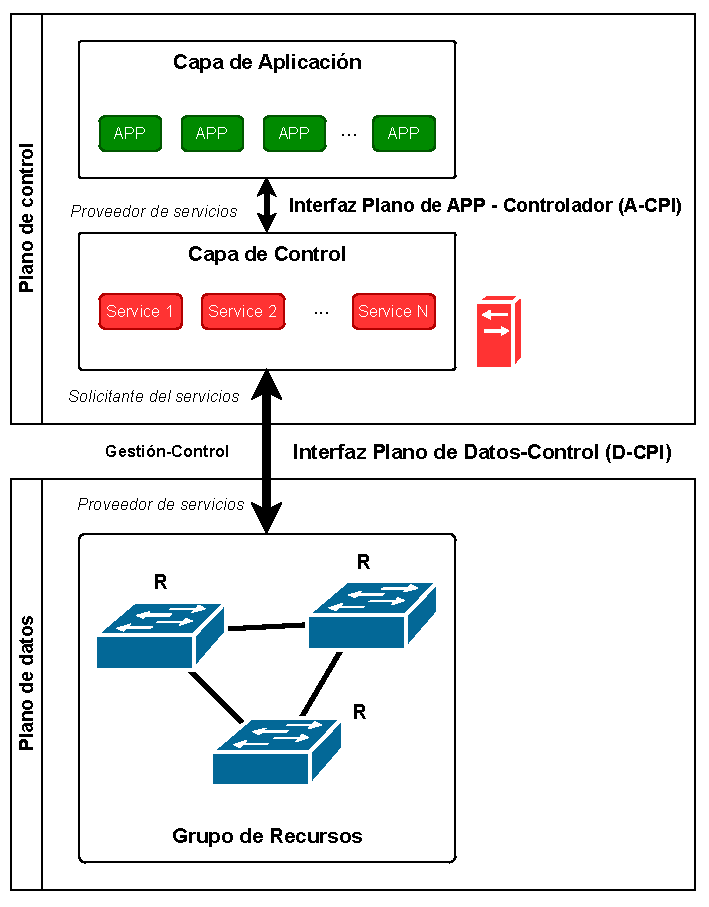
\includegraphics[width=0.65\textwidth]{fig/02_sota/sota_6_sdn_arch_mcc.drawio.pdf}
\caption{Paradigmas de control \emph{Management–Control Continuum} (MCC)}
\label{fig:sota_6_sdn_arch_mcc}
\end{figure}

Según la \gls{onf}, una arquitectura es una colección necesariamente incompleta de perspectivas sobre un conjunto de ideas subyacentes, por ello, partiendo del modelo básico de \gls{sdn}, trataron de identificar todas las funcionalidades que implementaba el controlador como servicios que gestionan una serie de recursos, en este caso los nodos de la red, llevando a la mínima expresión la arquitectura de una manera agnóstica, para que esta fuera extrapolable a cualquier tipo de redes programables y heterogéneas. Por ende, un consumidor de servicio, será aquel que intercambia tanto datos como operaciones de control y gestión con un servidor o proveedor \gls{sdn} (D-CPI).  Aunque los datos del usuario son finalmente transmitidos o procesados por un conjunto de recursos (R) que pertenecen al proveedor \gls{sdn}, el cliente final controla su servicio mediante una sesión de control y gestión, invocando acciones (A-CPI) sobre un conjunto de recursos virtuales alojados en el controlador que percibe como propios. El controlador \gls{sdn}, entre otras funciones, se encarga de virtualizar y orquestar la vista de recursos y servicios que tiene el cliente, mapeándola sobre los recursos y servicios reales del proveedor. Los conceptos de ``recursos'' y ``servicios'' son intencionalmente flexibles y no tienen límites fijos. La arquitectura \gls{sdn} amplía este modelo básico, al denominado como \gls{mcc}, y aclara sus implicaciones, incluyendo extensiones clave como el uso compartido de recursos entre múltiples clientes, la asignación dinámica y la optimización de su uso.\\
\\
El \gls{mcc} organiza las capacidades de la red en una jerarquía de servicios que va desde los servicios básicos de gestión y control (descubrimiento, provisión, configuración, monitorización) hasta servicios avanzados de orquestación y automatización que permiten funcionalidades de alto valor sobre infraestructuras softwarizadas. Esta visión facilita describir la red como una plataforma de servicios en la que la infraestructura subyacente se abstrae y se pone a disposición de funciones gestionadas y componibles. Bajo el paraguas del \gls{mcc}, resulta útil clasificar el estado del arte en dos bloques complementarios que recogen las tecnologías habilitantes principales que se exploran en esta Tesis: (i) servicios básicos que habilitan la operación mínima de la softwarización (descubrimiento de topología, arranque autónomo, provisión de canales de control, telemetría) y (ii) servicios avanzados que aportan capacidades de decisión, predicción y optimización (orquestación, planeamiento de recursos, predicción de fallos y adaptación proactiva), normalmente apoyados en técnicas de inteligencia artificial y aprendizaje automático. En las siguientes sub-Secciones, se explorarán los contenidos principales de esta Tesis englobados sobre los dos bloques de servicios anteriormente mencionados en el contexto del paradigma de control \gls{mcc}.


\subsection{Servicios básicos: arranque y provisión de canales de control en entornos densos y heterogéneos}
% intro, etiquetado jerarquico y rutas, tree en el root, conceptos de grafos (terminología básica)
% propuestas 
% sota tfm conf.
% sota den2de

Los servicios básicos de arranque y provisión de canales de control constituyen la base operativa del \gls{mcc}. Sin un mecanismo fiable para que los dispositivos descubran la topología, obtengan parámetros iniciales y establezcan conectividad con el controlador, es imposible desplegar servicios de mayor nivel. En entornos densos y heterogéneos (\gls{iiot}, micro-redes eléctricas, redes logísticas), las restricciones de recursos, la topologías multi-salto y la posible ausencia de enlaces dedicados obligan a diseñar protocolos \emph{in-band} o híbridos que sean escalables, seguros y poco intrusivos, a la par que resilientes.\\
\\
En la Sección~\ref{subsec:propuestas_inband} se pudo explorar todas las propuestas de mecanismos in-band, entre las cuales se pudo observar diferentes estrategias de arranque/provisión que emplea:

\begin{enumerate}
  \item \textbf{Protocolos clásicos asistidos (DHCP/ARP/LLDP):} usan servicios L2/L3 existentes para obtener parámetros y descubrir topología (p. ej. \cite{Sharma13}).
  
  \item \textbf{Árboles raíz-centrados y exploración por difusión:} el nodo raíz (con enlace al controlador) propaga paquetes de exploración que recogen topología y permiten instalar rutas in-band~\cite{Lopez-Pajares19}).
  
  \item \textbf{Etiquetado jerárquico:} asignación de identificadores temporales o jerárquicos a nodos para encaminar mensajes de control sin conocer la topología completa (p. ej. la propuesta de Izzy ~\cite{Holzmann19}).
  
  \item \textbf{Híbridos con canales out-of-band para arranque:} soluciones que requieren un enlace auxiliar o reglas preinstaladas para la fase inicial y luego migran a in-band (véase \cite{Gonzalez18,Su17}).
  
  \item \textbf{Mecanismos basados en multipath/TCP avanzado:} uso de \gls{mptcp} para mejorar disponibilidad del canal de control mediante rutas múltiples (p. ej. \cite{Raza17}).
  
\end{enumerate}

Sin embargo, gran parte de las soluciones revisadas fueron concebidas para redes de comunicaciones convencionales y, como consecuencia, dependen de protocolos auxiliares o de implementaciones específicas en equipos \gls{sdn}. Ese fuerte acoplamiento limita su aplicabilidad a entornos densos y heterogéneos, por ejemplo, redes con nodos de recursos muy reducidos (\gls{iiot}) o redes de distribución eléctrica con topologías en árbol, donde no es viable confiar en servicios adicionales ni en modificaciones de hardware/software. En contraste, los enfoques más abstractos, basados en esquemas de etiquetado jerárquico y en la construcción de árboles enraizados combinados con mecanismos de difusión/control de exploración, resultan más extrapolables y prácticos para estos escenarios: reducen dependencias infraestructurales, facilitan la escalabilidad y favorecen la resiliencia mediante rutas alternativas y reconvergencia local, por lo que constituyen las candidatas más adecuadas para los objetivos de esta Tesis.\\
\\
Los esquemas basados en etiquetado jerárquico combinados con la construcción de árboles enraizados constituyen una estrategia natural y eficiente para el arranque y la provisión de canales de control en redes densas y heterogéneas. En estos enfoques, la red se organiza lógica o temporalmente en niveles mediante identificadores (etiquetas) que codifican información de pertenencia o proximidad, de forma análoga a prefijos jerárquicos; dichas etiquetas permiten encaminar mensajes de control con mínimo conocimiento global, reduciendo la necesidad de tablas extensas en los nodos. Estas etiquetas, pueden identificar a nivel de nodo, a nivel de enlace o a nivel de puerto, y dependerá del caso de uso que tipo de identificador emplear. La construcción de un árbol enraizado con la raíz colocada en el nodo, o nodos, con acceso directo al controlador facilita el arranque de la red, dado que, paquetes de exploración pueden propagarse de forma controlada desde la raíz acumulando información topológica y asignando rutas in-band sin inundar la red. Esta combinación aporta ventajas prácticas relevantes para entornos con recursos limitados: localiza las decisiones de reencaminamiento, ofrece caminos de protección natural (rutas alternativas hacia la raíz dentro del árbol o a través de etiquetas vecinas) y limita el \textit{overhead} de señalización. No obstante, conlleva retos propios, como por ejemplo, la gestión dinámica de etiquetas ante cambios topológicos (re-etiquetado) puede generar coste de señalización, y es preciso diseñar mecanismos para evitar bucles y ataques por suplantación (p. ej. autenticación ligera de mensajes de exploración). Es por ello, que el etiquetado jerárquico más árboles enraizados proporciona un marco abstracto, escalable y resistente, bien adaptado a \gls{iiot}, micro-redes y topologías jerárquicas en árbol típicas en redes de distribución eléctrica, siempre que se complemente con políticas de convergencia eficientes y escalables adecuadas para el caso de uso final.\\
\\
Para analizar con mayor detalle los enfoques basados en etiquetado jerárquico y la construcción de árboles enraizados, esta sección introduce los conceptos básicos de teoría de grafos necesarios para modelar la topología de una red y para explicar cómo, mediante esquemas de etiquetado, es posible derivar una estructura de árbol enraizado adecuada para el arranque y el encaminamiento de control. A continuación se formalizan los términos y notaciones que se emplearán en el resto del capítulo; posteriormente se estudian diferentes propuestas de etiquetado jerárquico y su aplicabilidad a las redes densas y heterogéneas.  

\subsubsection{Terminología básica}

La teoría de grafos es la disciplina matemática que estudia las propiedades y estructuras de los grafos. Un grafo es una representación visual compuesta por una serie de objetos llamados nodos, conectados a través de otro tipo de objetos denominados enlaces. Históricamente, los orígenes de la teoría de grafos se remontan al problema de los puentes de Königsberg, también conocido como problema de los siete puentes de Königsberg. Su nombre se debe al nombre de la ciudad, Königsberg, ciudad de Prusia Oriental, y el problema consistía en encontrar un camino para cruzar a pie toda la ciudad pasando solo una vez por cada uno de los siete puentes y regresando al mismo punto de partida. El problema, formulado originalmente de manera informal, se propagó a modo de juego matemático entre los intelectuales de la época, siendo resuelto por Leonhard Euler en 1736~\cite{euler1741solutio} y cuya resolución dio origen  y sentó las bases de la teoría de grafos.\\
\\
Formalmente, un grafo se define como $G \: = \: (\mathcal{N}, \mathcal{L})$, siendo  $\mathcal{N}$ un conjunto de $N$ nodos, y $\mathcal{L} \subseteq \{\{i,j\} \: | \: i,j \in \mathcal{N} \: con \: i \neq j\}$, un conjunto de enlaces los cuales se componen de un par desordenado de nodos, es decir, cada enlace tiene dos nodos diferentes. Estos enlaces pueden tener una direccionalidad, o no.  Atendiendo a la direccionalidad del conjunto de enlaces, los grafos se pueden clasificar en grafos dirigidos o no dirigidos, siendo los grafos dirigidos los que restringen el tránsito por los enlaces a una o varias direcciones específicas, mientras que los grafos no dirigidos no establecen ninguna obligatoriedad en la dirección de tránsito. Asimismo, se puede establecer un coste asociado a atravesar un enlace, pudiendo clasificar los grafos también en grafos ponderados, donde los enlaces tienen un coste asociado, y no ponderados, donde los enlaces no cuentan con un coste asociado. Otra característica interesante para clasificar los grafos es si tienen ciclos (bucles) o no. Un grafo se considera acíclico si no contiene ningún ciclo, esto significa que para cada nodo $i \in \mathcal{N}$, no hay un camino directo que empiece y termine en $i$.\\
\\
Si, además, es conexo y no dirigido, es decir, existe un camino entre cualquier par de nodos, y acíclico, se denomina árbol. En el caso dirigido, cuando no existen ciclos dirigidos se habla de un \gls{dag}. La presencia o ausencia de ciclos es una propiedad estructural clave que condiciona los algoritmos de encaminamiento, los procesos de exploración/\textit{bootstrapping} y los mecanismos de convergencia (por ejemplo, la prevención de bucles o la estrategia de etiquetado). Por ello, su consideración resulta esencial en el diseño de esquemas de etiquetado jerárquico y en la derivación de árboles enraizados a partir de la topología original \(G\).\\
\\
Por tanto, la teoría de grafos se puede aplicar de forma directa sobre las redes densas y heterogéneas, modelando dichas redes partiendo de una topología física a un grafo, el cual será hiperconectivo. Sobre la topología física habrá que definir cual será el nodo, o los nodos, que darán acceso al controlador, los cuales se identificarán como nodos raíz. Dichos nodos serán los encargados de iniciar el establecimiento del proceso de etiquetado jerárquico para poder construir el árbol enraizado. Este árbol, según se ha indicado, es un tipo especial de grafo acíclico conectado, el cual, también puede considerarse como un grafo con $n$ nodos y $n-1$ enlaces. Esto se puede analizar como la construcción de una topología lógica sobre una topología física, la cual contendrá todos los nodos de la topología anterior, pero un subconjunto de los enlaces de la topología física. Formulando este proceso del establecimiento de la topología lógica, podemos definir que dado un grafo $G \: = \: (\mathcal{N}, \mathcal{L})$, siendo  $\mathcal{N}$ un conjunto de $N$ nodos y $\mathcal{L} \subseteq \{\{i,j\} \: | \: i,j \in \mathcal{N} \: con \: i \neq j\}$ un conjunto de enlaces los cuales se componen de un par desordenado de nodos (es decir, cada enlace tiene dos nodos distintos), se puede obtener la topología lógica como un subgrafo, sea $G' \: = \: (\mathcal{N}', \mathcal{L}')$ donde se que cumple $\mathcal{N}' \subseteq \mathcal{N}$ y $\mathcal{L}' \subseteq \mathcal{L}$. En este caso, de forma adicional, se cumple la relación de igualdad para los nodos, dado que $\mathcal{N}' \subseteq \mathcal{N} \: \wedge \: \mathcal{N} \subseteq \mathcal{N}' $, haciendo que $\mathcal{N}' \: = \: \mathcal{N}$. Es decir, $a_{i} \in \mathcal{N} \: / \: b_{i} \in \mathcal{N}'$, $0 \leq i \leq N$ se cumple $\forall \: a_{i} \: = \: b_{i}$.\\
\\
Para ilustrar este proceso de establecimiento de la topología lógica, se presenta la Figura \ref{fig:topo_logic_1}. Como se puede ver en la Figura \ref{fig:topo_logic_1} (a), se parte de un grafo inicial, el cual representará a pequeña escala una red densa y heterogénea. Sobre este grafo se pueden seleccionar distintos subgrafos que cumplan la relación de igualdad según se ha explicado anteriormente. Pudiendo elegir entre distintas topologías lógicas (b,c,d) a conveniencia, y función de que nodo se establezca como nodo raíz de la topología. En el caso de que el nodo raíz de la topología fuera el nodo \textit{1}, podemos seleccionar la topología lógica (b) que habilita al nodo \textit{5} de una conexión más directa con el nodo que da acceso al controlador. Otra opción sería elegir la configuración (c), en caso de que los nodos \textit{5} y \textit{6} no tuvieran una necesidad explicita \gls{qos} en la comunicación con el controlador de la red.  De igual forma podemos elegir otra configuración, como por ejemplo (d), donde el nodo \textit{4} se encontrara al final de la topología lineal conformada. La elección concreta de la topología lógica, y por tanto la forma del árbol enraizado, depende de criterios de diseño del caso de uso. Por ejemplo, minimizar la profundidad del árbol (para reducir latencias hacia la raíz), priorizar enlaces con mayor capacidad o menor pérdida (criterio \gls{qos}), favorecer rutas disjuntas para aumentar la resiliencia, o minimizar el overhead de señalización. 

\begin{figure}[ht!]
   \centering
   \includegraphics[width=\textwidth]{fig/02_sota/sota_7_topo_logic_1.eps}
   \caption{Elección de una topología lógica (árbol enraizado) partiendo una topología física}
   \label{fig:topo_logic_1}
\end{figure}


El etiquetado jerárquico es una técnica eficiente y abstracta para obtener una topología lógica, habitualmente un árbol enraizado, a partir de una topología física \(G=(\mathcal{N},\mathcal{L})\). En este paradigma, a cada nodo \(i\in\mathcal{N}\) se le asigna una etiqueta que codifica su posición relativa dentro de una jerarquía o partición de la red. Estas etiquetas permiten a los nodos tomar decisiones de reenvío locales, por ejemplo, mediante coincidencia de prefijos, sin requerir una visión global completa de \(G\). El etiquetado jerárquico resulta especialmente adecuado para entornos densos y heterogéneos porque reduce la información de estado requerida en nodos con recursos limitados, facilita la derivación de rutas hacia la raíz o raíces usando información local y habilita mecanismos de agregación que simplifican la gestión. Existen diversas familias de esquemas de etiquetado jerárquico. En el etiquetado por prefijos, cada etiqueta se expresa como una secuencia jerárquica \(i_1.i_2. \dots .i_k\). En el etiquetado por intervalos, a cada subárbol o partición se le asigna un intervalo de identificadores, de modo que un nodo conoce su pertenencia comprobando si su identificador está dentro del intervalo correspondiente. Otros enfoques utilizan identificadores compactos que codifican información relativa a la distancia o la topología respecto a la raíz, y todavía existen esquemas basados en clusterización, en los que la red se divide en grupos y cada grupo recibe una etiqueta de nivel superior con subetiquetas internas. La elección entre estas variantes suele depender de limitaciones de memoria, de la necesidad de agregar información (p. ej. capacidades o requisitos \gls{qos}) y de la facilidad de reconfiguración en caso de cambios topológicos.\\
\\
Operativamente, la creación de la topología lógica mediante etiquetado se articula en varias fases. Primero se seleccionan las raíces, es decir, los nodos con acceso directo al controlador o controladores, que actuarán como iniciadores del proceso. A continuación, desde la raíz se emiten mensajes de exploración controlada que se propagan por la red física; al recibir un mensaje por primera vez, un nodo acepta la etiqueta propuesta (por ejemplo, concatenando un identificador del enlace, el puerto, su identificador o un sufijo jerárquico) y establece una relación ``vecindad'' con el emisor. Con la etiqueta asignada, cada nodo obtiene reglas locales de reenvío que permitan encaminar paquetes de control hacia su padre y, por ende, hacia la raíz. De forma complementaria, es posible manejar varias etiquetas por nodo que identifiquen rutas alternativas, facilitando así la reconvergencia rápida ante fallos de enlace o de nodo. En entornos prácticos, estas fases deben diseñarse para evitar inundaciones de mensajes y para que la aceptación de etiquetas siga políticas antibucles.\\
\\
Para ilustrar este proceso se presenta la Figura~\ref{fig:sota_8_topo_difusion_1}. En este caso se puede apreciar un grafo de cinco nodos, entre los cuales se ha elegido al nodo \textit{1} como nodo raíz de la topología. Será este nodo quien empiece el proceso de difusión del etiquetado jerárquico. En este escenario se ha optado por un tipo de etiquetado basado en identificadores únicos los cuales representan de forma inequívoca al nodo dentro de la topología física. En el primer paso de la difusión, ver  Figura~\ref{fig:sota_8_topo_difusion_1} (a), el nodo raíz empieza a difundir su etiqueta con identificador único \texttt{1}, la cual llega hasta el nodo \textit{2}, quien la recibe y acto seguido concatena su identificador único generando la etiqueta \texttt{1.2} que será almacenada y difundida por todos los enlaces disponibles menos por el que le llego (siendo un aspecto de diseño en la estrategia de etiquetado). De forma análoga, el nodo \textit{3} generará la etiqueta \texttt{1.2.3}, almacenándola y difundiéndola a los nodos \textit{4} y \textit{5}, obteniendo estos a su vez las etiquetas \texttt{1.2.3.4} y \texttt{1.2.3.5}, respectivamente. En el segundo paso de la difusión, ver  Figura~\ref{fig:sota_8_topo_difusion_1} (b), los nodos de la topología ya tienen un camino directo para alcanzar el nodo raíz, el nodo \textit{2} de forma directa, el nodo \textit{3} a través del nodo \textit{2}, y los nodos \textit{4} y \textit{5} a través del nodo \textit{3}. Sin embargo, el proceso de difusión no ha concluido, dado que los nodos \textit{4} y \textit{5} aún tienen una etiqueta por difundir, la cual se intercambian entre ellos. En el tercer paso de la difusión, ver  Figura~\ref{fig:sota_8_topo_difusion_1} (c), los nodos \textit{4} y \textit{5} obtienen las etiquetas \texttt{1.2.3.5.4} y \texttt{1.2.3.4.5} respectivamente, lo que les habilita a una ruta adicional hacia el nodo raíz (del nodo \textit{4} a través del nodo \textit{5}, y viceversa), pudiendo elegir entre un camino u otro.  

\begin{figure}[ht!]
   \centering
   \includegraphics[width=\textwidth]{fig/02_sota/sota_8_topo_difusion_1.eps}
   \caption{Ejemplo de difusión empleando el etiquetado jerárquico}
   \label{fig:sota_8_topo_difusion_1}
\end{figure}

En el último paso (Figura~\ref{fig:sota_8_topo_difusion_1} (c)), se puede apreciar otro aspecto clave de los esquemas de etiquetado: los mecanismos antibucle. Los nodos \textit{4} y \textit{5} reciben respectivamente las etiquetas \texttt{1.2.3.5.4} y \texttt{1.2.3.4.5}, la cuales tendrán que ser difundidas de forma análoga hacia el nodo \textit{3}. Al llegar dichas etiquetas al nodo \textit{3}, y al utilizar identificadores inequívocos, este tiene la capacidad de comprobar si las etiquetas recibidas contienen su propio identificador, y en tal caso descartarlas, dado que en propio significado de la etiqueta le estaría indicando al nodo que en esa ruta tendría que volver sobre el en una ocasión, reflejando un bucle (ciclo). Una vez descartadas las etiquetas, y con todas las etiquetas difundidas en la topología física, todos los nodos tendrían una o más rutas para alcanzar al nodo raíz y conocerían su posición jerárquica en la topología. De esta forma, aplicando diferentes criterios de los anteriormente mencionados, se podrían obtener tres topologías lógicas (tres arboles) a partir de una topología física: el primero donde los nodos \textit{4} y \textit{5} cuelgan directamente del nodo \textit{3}, el segundo donde el nodo \textit{4} se conecta directamente al nodo \textit{3} y el nodo \textit{5} se conecta al nodo \textit{4}, y el tercero, donde el nodo \textit{5} se conecta directamente al nodo \textit{3} y el nodo \textit{4} se conecta al nodo \textit{5}. Este proceso de etiquetado y selección de la topología lógica puede ser ejecutando de forma periódica, o configurable, para actualizar el encaminamiento automático, explorar de nuevo la topología en escenarios de movilidad o modificaciones de la topología física, siendo esto critico en redes densas y heterogéneas.\\
\\
El diseño de esquemas de etiquetado implica una serie de \textit{trade-offs} relevantes. Etiquetas más compactas reducen la memoria y la carga de procesamiento en los nodos, pero limitan la información codificable (por ejemplo, la posibilidad de transportar metadatos de capacidad o prioridad). Los esquemas por prefijo e intervalos son naturalmente agregables y escalables, pero pueden requerir re-etiquetado amplio cuando la topología cambia; por ello, las soluciones prácticas suelen implementar re-etiquetado localizado, versionado de etiquetas o etiquetas temporales para mitigar la señalización. La prevención de bucles durante la fase de construcción exige políticas en los mensajes de exploración según se ha indicado.\\
\\
Es por ello, que el etiquetado jerárquico encaja especialmente bien con los requisitos de redes \gls{iiot}, micro-redes y sistemas de distribución eléctrica y redes de comunicaciones, dado permite realizar \textit{bootstrapping} sin depender de servicios L2/L3 adicionales ni de extensiones propietarias, limita el estado necesario en cada nodo, escala bien con el tamaño de la topología física, y facilita la introducción explícita de rutas de respaldo. Además, este enfoque se complementa de forma natural con técnicas de \gls{ai}/\gls{ml}, modelos predictivos pueden priorizar la exploración de determinados subárboles, seleccionar enlaces con menor probabilidad de fallo o recomendar políticas de re-etiquetado que optimicen la resiliencia y el rendimiento de la topología lógica. En la siguiente sección, se analizarán algunas de las propuestas de etiquetado jerárquico, se compararán sus prestaciones y bondades que serán de utilidad en los entornos estudiados en esta Tesis.



\subsubsection{Propuestas de etiquetado jerárquico}
\label{subsubsec:propuestas_etiquetado}

En el contexto de los servicios básicos, en concreto, al arranque y provisión de canales de control en entornos densos y heterogéneos, el etiquetado jerárquico aparece como una solución consolidada dentro del catálogo de funcionalidades que el \gls{mcc} clasifica como servicios de gestión y control fundamentales. Aunque el etiquetado jerárquico no constituye una novedad conceptual~\cite{fraigniaud2000assigning}, ha sido aplicado con éxito en dominios tan diversos como enrutamiento por prefijos~\cite{rojas2012torii}, direccionamiento en redes de sensores y esquemas de localización para \gls{iot}~\cite{rojas2021outperforming}, su carácter transversal y su capacidad de abstracción lo convierten en un mecanismo idóneo para materializar las capacidades mínimas que exige el \gls{mcc} en escenarios con recursos limitados y topologías heterogéneas. Por otra parte, muchas de las propuestas y variaciones prácticas que se examinan a continuación proceden de nuestro grupo de investigación, NetIS, que lleva años investigando y prototipando esquemas de etiquetado y árboles enraizados; estas aportaciones servirán de referencia a la hora de comparar enfoques, identificar \textit{gaps} y situar las contribuciones de esta Tesis en el marco de las redes densas y heterogéneas. A continuación se presenta una taxonomía de enfoques y se analizan propuestas representativas, prestando especial atención a su aplicabilidad práctica, requisitos de implementación y limitaciones en entornos densos, distribuidos y heterogéneos.\\
\\
En primer lugar, los trabajos teóricos clásicos proporcionan la base formal del problema de asignación de identificadores en redes anónimas. Uno de los primeros trabajos identificados en materia de etiquetado jerárquico lo presentan Fraigniaud \textit{et al.}~\cite{fraigniaud2000assigning}, donde estudian la asignación de etiquetas únicas en redes anónimas sin conocimiento previo de la topología ni de su tamaño, empleando un modelo síncrono con una fuente distinguida, un nodo raíz, que inicia el proceso. Sus resultados son valiosos porque demuestran límites y \textit{trade-offs} fundamentales entre longitud de etiqueta, tiempo y complejidad de mensajes; sin embargo, las fuertes hipótesis (p. ej. sincronía estricta) y la ausencia de tratamiento de topologías dinámicas o con fallos hacen que su aplicabilidad directa a entornos reales y heterogéneos sea limitada. Este tipo de trabajo marca el terreno teórico, pero deja abiertos problemas prácticos como la asincronía y las restricciones de recursos en redes de baja capacidad.\\
\\
En el ámbito aplicado, una familia de propuestas orientadas a los \gls{dc} explora mecanismos de etiquetado jerárquico para encaminamiento sin tablas y reenvío rápido. Rojas \textit{et al.}~\cite{rojas2012torii}, presentan Torii-HLMAC, donde introducen direcciones posicionales, \gls{hlmac}, y un mecanismo distribuido de asignación automática que habilita encaminamiento sin tablas en \textit{bridges} y recuperación instantánea ante fallos. Más adelante, Rojas \textit{et al.}~\cite{rojas2017ga3,rojas2021scalable}, evolucionan esta idea, presentando \gls{ga3} y eTorii. \gls{ga3} propone un descubrimiento distribuido que genera múltiples direcciones \gls{hlmac} ordenadas y soporta encaminamiento sin tablas de reenvío sobre árboles de rutas mínimas; eTorii combina \textit{source routing} con asignación automática para permitir encaminamiento \textit{on-the-fly}. Estas propuestas comparten ventajas claras para topologías jerárquicas (baja ocupación de estado, conmutación rápida, balanceo por selección de etiquetas), pero su evaluación se ha centrado mayoritariamente en topologías de \gls{dc} (fat-trees, topologías jerárquicas) y bajo condiciones relativamente homogéneas. Por ello, se pueden identificar una serie de debilidades evidentes, como por ejemplo, la extrapolación a topologías irregulares o muy heterogéneas, el comportamiento bajo enlaces de muy distinta capacidad/latencia, y el coste de implementación en dispositivos con capacidades limitadas requieren más estudio experimental y, en algunos casos, soporte en hardware (p. ej. \gls{p4}) para validar su uso en producción.\\
\\
En paralelo aparecen soluciones probabilísticas y adaptativas pensadas para redes dinámicas. El trabajo publicado por Walraed \textit{et al.}~\cite{walraed2013randomized}, presentan la solución ALIAS bajo el protocolo \textit{Decider/Chooser Protocol} (DCP), donde proponen algoritmos aleatorizados para la selección de etiquetas en redes con cambios frecuentes; su fortaleza es la adaptabilidad y las buenas garantías probabilísticas de convergencia, pero su evaluación se centra en escenarios de centros de datos y deja abierto cómo se comporta en entornos con recursos muy limitados o con tasas extremas de \textit{churn} (tasa de abandono y unión masiva de nodos). Estos enfoques aleatorizados aportan resiliencia frente a dinamismo, pero su sobrecoste de mensajes y su idoneidad para nodos de baja energía deben cuantificarse para \gls{iiot}.\\
\\
Respecto a redes de baja capacidad con restricciones en consumo, y en almacenamiento de información de estado, Rojas \textit{et al.}~\cite{rojas2021outperforming}, presentan IoTorii, donde se adapta el paradigma jerárquico a las \gls{llns}. IoTorii se basa también en las \gls{hlmac}, reutilizando direcciones MAC típicas transformándolas en etiquetas jerárquicas y emplea sondas \textit{broadcast} para descubrir rutas múltiples sin modificar la pila de protocolos utilizada en las \gls{llns}. Los resultados experimentales muestran reducción de entradas en tablas de reenvío, y un menor \textit{overhead} respecto a \gls{rpl} (protocolo de facto en las \gls{llns}) en escenarios estáticos, lo que evidencia la promesa del etiquetado en entornos de baja potencia. No obstante, quedan sin resolver la robustez ante movilidad elevada, la variabilidad extrema de enlaces y la necesidad de políticas energéticas más agresivas para redes de sensores reales, densas y heterogéneas.\\
\\
En cuanto a las soluciones enfocadas directamente a las redes típicas \gls{sdn}, tenemos que volver a mencionar Lopez-Pajares \textit{et al.}~\cite{Lopez-Pajares19}, y Holzmann \textit{et al.}~\cite{Holzmann19}, vistos en la Sección~\ref{subsec:propuestas_inband}, pero haciendo ahora hincapié en su enfoque de etiquetado jerárquico. Lopez-Pajares \textit{et al.}~\cite{Lopez-Pajares19}, presentaban Amaru, donde apuestan por la exploración controlada desde un nodo raíz para recopilar topología e instalar rutas in-band. Amaru combina exploración y construcción de rutas con respaldo múltiples, y demuestra tiempos de recuperación muy bajos con \textit{overhead} casi nulo. El etiquetado que emplean se basa en los identificadores de los puertos de los nodos \gls{sdn} que gestionan, haciendo que su principal limitación práctica es que requiere ligeras modificaciones en los switches \gls{sdn} para soportar el protocolo, lo que plantea barreras de despliegue en entornos heterogéneos donde no es posible modificar el plano de datos de todos los equipos. Este es un debilidad operativa importante para entornos industriales o de infraestructura crítica donde la interoperabilidad con equipos \textit{legacy} es necesaria. De forma similar, Holzmann \textit{et al.}~\cite{Holzmann19}, proponen Izzy, basado en un un diseño modular, que combina un árbol de expansión con identificadores temporales dependientes de la topología para asegurar conectividad in-band con tiempos de recuperación por debajo de 100 ms en simulaciones de \gls{wan}. Los identificadores temporales les ayudan a detectar cuando uno de los nodos establecidos en la ruta in-band deja de estar operativo, lo que les permite actualizar dichas rutas y reparar el canal de comunicación en un tiempo adecuado. Izzy aporta una arquitectura bien estructurada para mantener tablas y rutas de respaldo, y demuestra que la combinación etiquetado junto al árbol de expansión puede alcanzar latencias de conmutación muy bajas. Sin embargo, su validación está limitada a simulación y queda por demostrar su factibilidad en despliegues heterogéneos reales; además, la generación y gestión de identificadores temporales plantea cuestiones de coordinación entre controladores en escenarios multi-root, es decir, donde hay más de un nodo con acceso al controlador \gls{sdn}.\\
\\
Recapitulando y comparando, todos los trabajos explotan la idea común de codificar información topológica en etiquetas jerarquicas para reducir estado local y facilitar el encaminamiento hacia la raíz, pero difieren en decisiones de diseño clave: (i) si la asignación es determinista (prefijos ordenados, intervalos) o probabilística; (ii) si el encaminamiento es sin tabla de reenvío (Torii/GA3) o requiere reglas instaladas (Amaru/Izzy); (iii) si la solución requiere o no modificaciones en el dataplane; y (iv) el alcance de la evaluación (simulación vs. prototipo vs. despliegue sobre hardware). Esos ejes determinan la aplicabilidad a entornos densos y heterogéneos: por ejemplo, las soluciones sin tabla de reenvío son atractivas para switches con escaso \gls{tcam}, pero su robustez en enlaces heterogéneos no ha sido ampliamente probada; las soluciones que requieren cambios en switches presentan una barrera de adopción en infraestructuras mixtas; las propuestas probabilísticas toleran \textit{churn} pero su coste de señalización puede ser alto para sensores con baterías limitadas.

\subsubsection{Conclusiones y alineación con los objetivos de la Tesis}

El análisis del estado del arte ha puesto de manifiesto que el etiquetado jerárquico y las técnicas basadas en árboles enraizados constituyen un marco fértil y consolidado para abordar el arranque y la provisión de canales de control en entornos densos y heterogéneos. Las propuestas revisadas (trabajos teóricos sobre asignación de identificadores, protocolos para centros de datos como Torii/GA3/eTorii, soluciones adaptadas a \gls{llns} como IoTorii, protocolos in-band como Amaru e implementaciones modulares como Izzy) comparten la idea de explotar información codificada localmente en etiquetas para reducir estado y facilitar encaminamiento hacia la raíz o raíces. Sin embargo, de la comparación sistemática emergen limitaciones claras en relación con el objetivo de aplicar estas técnicas fuera del dominio clásico de las redes de comunicaciones. Muchas soluciones se han validado únicamente en topologías jerárquicas homogéneas o en simulación, varias requieren modificaciones del \textit{dataplane} o soporte hardware específico, y pocas consideran nativamente la heterogeneidad de enlaces, la restricción de recursos de nodos \gls{iiot} o la coordinación multi-raíz entre controladores distribuidos.\\
\\
Esto encaja de forma directa con el planteamiento y los dos objetivos de la Tesis: (i) el estudio y diseño de algoritmos y mecanismos de control (etiquetado, encaminamiento, reconfiguración proactiva) aplicables a \gls{sdn}, \gls{iiot} y redes de distribución eléctrica; y (ii) el análisis de la infraestructura habilitadora (herramientas de despliegue y monitorización), incorporando técnicas de \gls{ai}/\gls{ml} como elemento auxiliar para predicción y toma de decisiones autónoma. En concreto, cada gap identificado se traduce en uno o varios posibles trabajos dentro de la Tesis: diseño de esquemas de etiquetado tolerantes a heterogeneidad, desarrollo de una capa de compatibilidad dataplane-agnóstica, protocolos de bootstrap ligeros, algoritmos de coordinación multi-raíz, y estudios que reduzcan la señalización en nodos con recursos limitados mediante decisiones locales haciendo uso del etiquetado jerárquico (posiblemente asistidas por técnicas de \gls{ai}/\gls{ml}). Estas líneas se integran de manera coherente con los objetivos generales de la Tesis y marcan un camino claro desde la revisión del estado del arte hacia contribuciones concretas, evaluables y orientadas a la transferencia tecnológica en contextos reales (IIoT, smart grids y otros entornos densos y heterogéneos).




\subsection{Servicios avanzados: gestión y planeamiento de recursos en entornos densos y heterogéneos}
% Intro
% Recursos de forma hetereogenas
% Terminología basica, centr

En esta subsección se revisan las capacidades avanzadas que, apoyadas en el \gls{mcc} y en las capas de orquestación, habilitan la gestión inteligible y el planeamiento de recursos en redes softwarizadas densas y heterogéneas. Estas capacidades van más allá de las funciones básicas de descubrimiento y provisión: incluyen la orquestación multi-capa (cloud/edge), la planificación de recursos con restricciones (computación, energía, latencia), mecanismos de autoscalado y balanceo, y técnicas de apoyo basadas en \gls{ai}/\gls{ml} para la predicción y la toma de decisiones proactiva. A continuación se propone una estructura detallada para abordar estos temas.


\subsection{Servicios avanzados: optimización y reconfiguración proactiva del control en entornos densos y heterogéneos}



\section{Casos de uso}  
\label{sec:casos_de_uso}
En este último bloque se revisan los casos de uso más relevantes que se pueden encontrar en la literatura. Estos casos de uso son ejemplos prácticos de cómo las tecnologías habilitantes y las redes programables y softwarizadas se aplican en contextos reales, como las \gls{sg} y las redes de sensores \gls{iiot}. 